\section{Circuiti}
\textbf{Nota bene: } la \textbf{differenza di potenziale/tensione($V$)} in parallelo non cambia, così come la \textbf{corrente($I$)} in serie non cambia.
\begin{gather*}
    \textbf{Differenza di Potenziale: } \\ V = I \cdot R \quad I = \frac{\Delta V}{R} \\
    \textbf{Potenza Dissipata: } \\
    W = I \cdot V = I^2 R = \frac{V^2}{R} \\
    \textbf{Condensatori: } \\ C = \frac{Q}{\Delta V}
\end{gather*}
\subsection{Leggi di Kirchhoff}
\begin{gather*}
    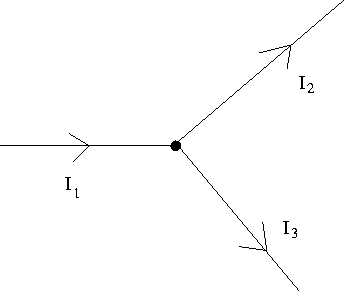
\includegraphics[width=0.7 \linewidth]{Circuiti/node_law.png} \\
    I_1 = I_3 + I_4 \\
    \textbf{Resistenze in serie: } \\
    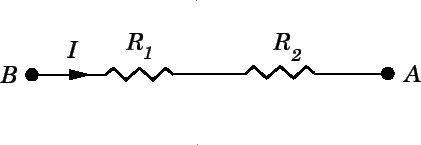
\includegraphics[width=0.75 \linewidth]    {Circuiti/resistenze_in_serie.png} \\ 
    R_{12} = R_1 + R_2 \\
    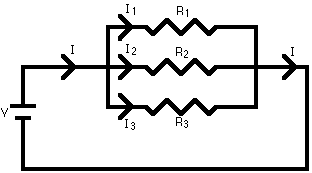
\includegraphics[width=0.75 \linewidth]    {Circuiti/resistenze_in_parallelo.png} \\
    \frac{1}{R_{123}} = \frac{1}{R_1} + \frac{1}{R_2} + \frac{1}{R_3} \\ \text{Oppure: } R_{123} = \frac{R_1 R_2 R_3}{R_1 + R_2 + R_3} \\
    \textbf{Condensatori in serie: } \\
    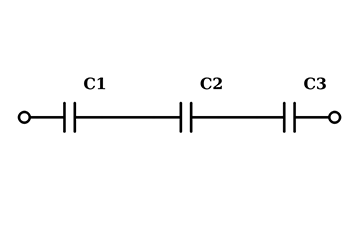
\includegraphics[width=0.75 \linewidth]    {Circuiti/condensatori_in_serie.png} \\
    \frac{1}{C_{123}} = \frac{1}{C_1} + \frac{1}{C_2} + \frac{1}{C_3} \\
    \text{Oppure: } C_{123} = \frac{C_1 C_2 C_3}{C_1 + C_2 + C_3} \\
    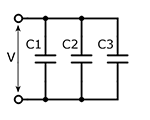
\includegraphics[width=0.75 \linewidth]    {Circuiti/condensatori_in_parallelo.png} \\
    C_{123} = C_1 + C_2 + C_3
\end{gather*}